\chapter{Modelagem}
\label{cap:modelagem}

Neste capítulo, as redes em malha sem fio são detalhadas através da descrição dos seus componentes. Depois, é apresentado como modelar uma rede usando grafos e como modelar as combinações de enlaces em uma árvore de combinações. 

Os modelos de iterferência são apresentados com o intuito de definir o teste de viabilidade e, futuramente, permitir algumas otimizações.

Ao final, é apresentado um exemplo de como enumerar os conjuntos viáveis ingenuamente usando os modelos introduzidos com Busca em Profundidade. As vantagens e desvantagens dessa abordagem são discutidas.

\section{Redes em Malha Sem Fio}
\label{section:mesh}

No capítulo anterior, foi definido que as Redes em Malha Sem Fio (WMN) são compostas por nós que podem funcionar como hosts ou roteadores. Isso quer dizer que os nós tanto executam uma aplicação, quanto auxiliam no rorteamento de pacotes. Além disso, os nós possuem rádios que são responsáveis pela transmissão e recepção no meio sem fio. Em uma WMN $\mathcal{R}$, o conjunto de nós é denotado por $\mathcal{N}$.

Nesse trabalho, é usado o modelo de propagação {\it log-distance}, no qual um sinal transmitido é atenuado por um fator que depende da distância entre o nó transmissor e o nó receptor. Todos os nós da rede transmitem a uma mesma potência de transmissão $PT$. Devido a esse modelo, o sinal transmitido por um nó $s$ é recebido em $r$ a uma potência de recepção $PR$, tal que $PR < PT$.

Se $PR$ for muito baixa, significa que a distância entre os nós é muito grande e os sinais recebidos provavelmente não poderão ser decodificados. É possível, então, definir uma distância máxima $\mathcal{D}$ entre um nó transmissor e um receptor, tal que a potência de recepção é mínima para que a mensagem possa ser decodificada. Quando um determinado nó $s \in \mathcal{N}$ transmite, qualquer nó $r \in \mathcal{N}$ que esteja dentro da área de transmissão centrada em $s$ e com do raio $\mathcal{D}$ consegue receber o sinal transmitido corretamente. Portanto, é possível estabelecer um enlace entre $s$ e $r$. Define-se o conjunto $\mathcal{L}$ contendo todos os enlaces estabelecidos dessa forma. 

\begin{figure}[htb]
\centering
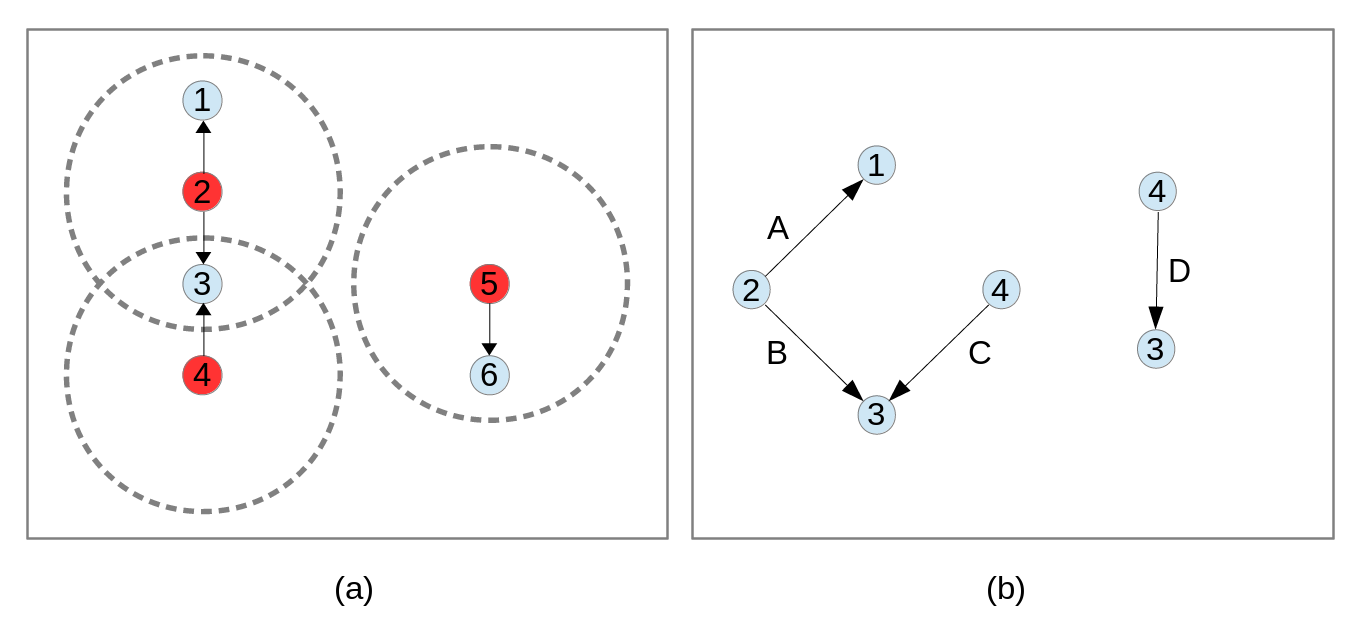
\includegraphics[width=1\textwidth]{figs/grafo}
\caption[Modelo da rede (a) usando o grafo (b).]
{Modelo da rede (a) usando o grafo (b).}
\label{fig:mesh}
\end{figure}

Na Figura \ref{fig:mesh}, um exemplo de uma rede simples com $|\mathcal{N}|=6$ nós e $|\mathcal{L}|=4$ enlaces é apresentado. Os nós 2, 4, e 5 estão ativos, ou seja, estão transmitindo, e os quatro enlaces são estabelecidos entre eles e os outros nós dentro de suas áreas de transmissão representadas pelo círculos sombreados. Como no caso do nó 3, é possível que nós estejam dentro de duas áreas de transmissão simultaneamente e, com isso, estejam participando de mais de um enlace como nó receptor. Simetricamente, caso mais de um nó esteja dentro da área de transmissão de um nó ativo, mais de um enlace podem ser estabelecidos, como no caso do nó 2. Não está ilustrado, mas também é possível que em um par de nós, ambos estejam ativos. Nesse caso, um enlace é definido em cada direção.

Devido a característica de {\it broadcast} em comunicações sem fio, caso um nó $s$ deseje transmitir a um nó $r$, o pacote será difundido através do meio físico e será interceptado por todos os nós da rede. Cada nó receberá o sinal transmitido a uma potência $PR$ que depende da distância até $s$. Para qualquer nó $u$, tal que $u \neq s,r$, a $PR$ a qual $u$ recebe o sinal de $s$ é definida como a interferência que $s$ causa em $r$. Em cenário com diversas transmissões ocorrendo, a coexistência dos enlaces formados a partir das transmissões no mesmo intervalo de tempo pode fazer com que os nós ativos em um enlace interfiram nos demais nós da rede, podendo prejudicar a comunicação. Ainda na Figura \ref{fig:mesh}, as setas tracejadas representam a interferência exercida por um transmissor em outros nós da rede.

Na seção \ref{section:interference} serão fornecidos mais detalhes sobre o modelo de propação log-distance e os modelos de interfência.

\section{Modelagem em Grafos}
\label{section:graphs}

Para modelar uma rede qualquer usando um grafo $G=(V,E)$, basta fazer as seguintes representações: os nós da rede são os vértices do grafo, ou seja constituem o conjunto $V(G)$ e, por convenção, $|V(G)|=n$; e os enlaces da rede são as arestas do grafo, ou seja constituem o conjunto $E(G)$ e, por convenção, $|E(G)|=m$.

Para esse trabalho, é importante que as arestas de G sejam direcionadas já que os enlaces especificam a direção da comunicação em um dado intervalo de tempo. A Figura \ref{fig:grafo} mostra um exemplo de como tal modelagem pode ser feita para a rede $\mathcal{R}$ da seção anterior usando um grafo $G=(V,E)$. Nesse caso, $\mathcal{N} \equiv V(G)$ e $\mathcal{L} \equiv E(G)$.

\begin{figure}[htb]
\centering
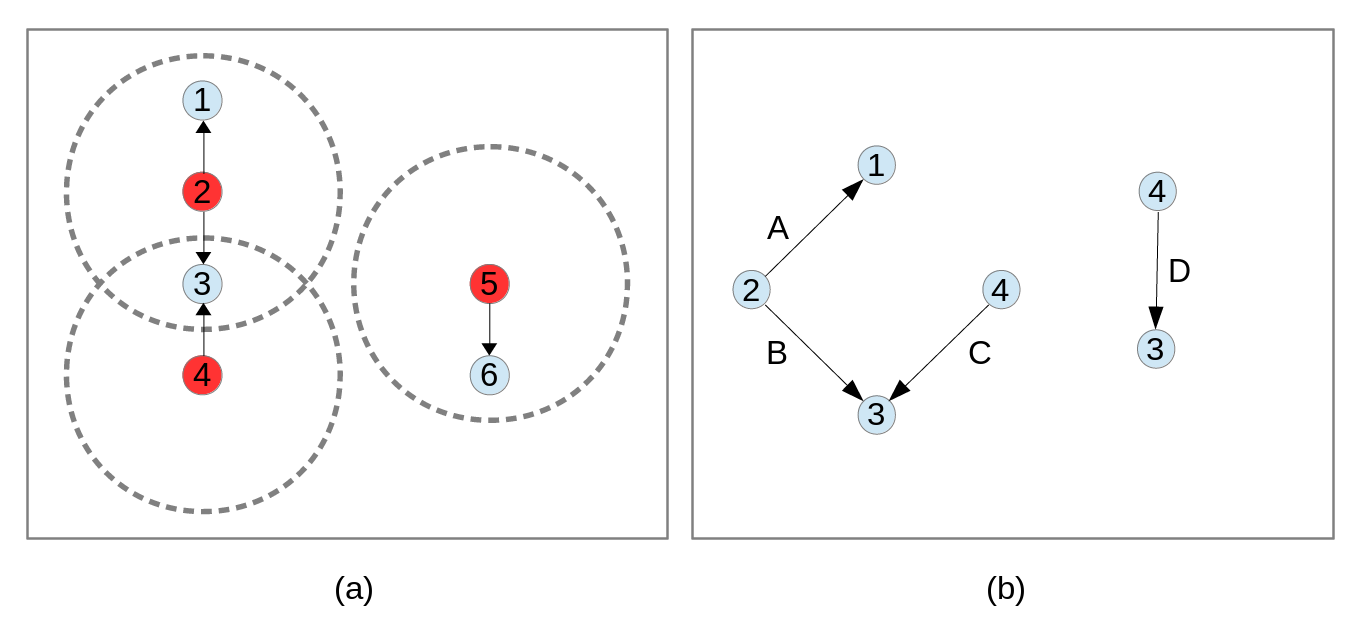
\includegraphics[width=1\textwidth]{figs/grafo}
\caption[Modelo da rede (a) usando o grafo (b).]
{Modelo da rede (a) usando o grafo (b).}
\label{fig:grafo}
\end{figure}

Modelar uma rede como um grafo é bastante útil pois permite utilizar algumas propriedades importantes da Teoria dos Grafos e fazer diversas manipulações matemáticas. Em especial, o uso de grafos ajuda a entender o modelo de interferência primária, discutido ainda nesse capítulo, e as otimizações baseadas em acoplamentos, introduzidas no capítulo \ref{cap:resultados}. Especificamente, nesse trabalho, a abstração em grafos também ajudou muito na etapa de implementação dos algoritmos.

\section{Árvore de Combinações}
\label{section:trees}

É possível definir um conjunto $C$, tal que $C \subseteq \mathcal{L}$, isto é, $C$ é uma combinação dos enlaces de $\mathcal{L}$. Com isso, tem-se que o menor tamanho de $C$ é zero, ou seja, não há enlaces ativos ($C=\emptyset$), e o maior tamanho é o próprio $\mathcal{L}$, com todos os enlaces possíveis ativos ($C=\mathcal{L}$). Se $|\mathcal{L}|=m$, usando a convenção da seção anterior, entre os dois extremos, existem $2^m$ combinações de enlaces possíveis, que são subconjuntos de $\mathcal{L}$ definidos pela escolha de quais enlaces estão ativos.

Sobre essas combinações de enlaces é possível definir uma árvore de combinações $A=(V,E)$. Os vértices da árvore são todas as combinações possíveis dos enlaces em $\mathcal{L}$. As arestas da árvore ligam qualquer combinação em uma altura $h$ a outra combinação em uma altura $h+1$ que pode ser obtido através da adição de um enlace de $E(G)$. Em $A$, o tamanho de uma combinação C a uma altura h na árvore é tal que $|C|=h$.

\begin{figure}[htb]
\centering
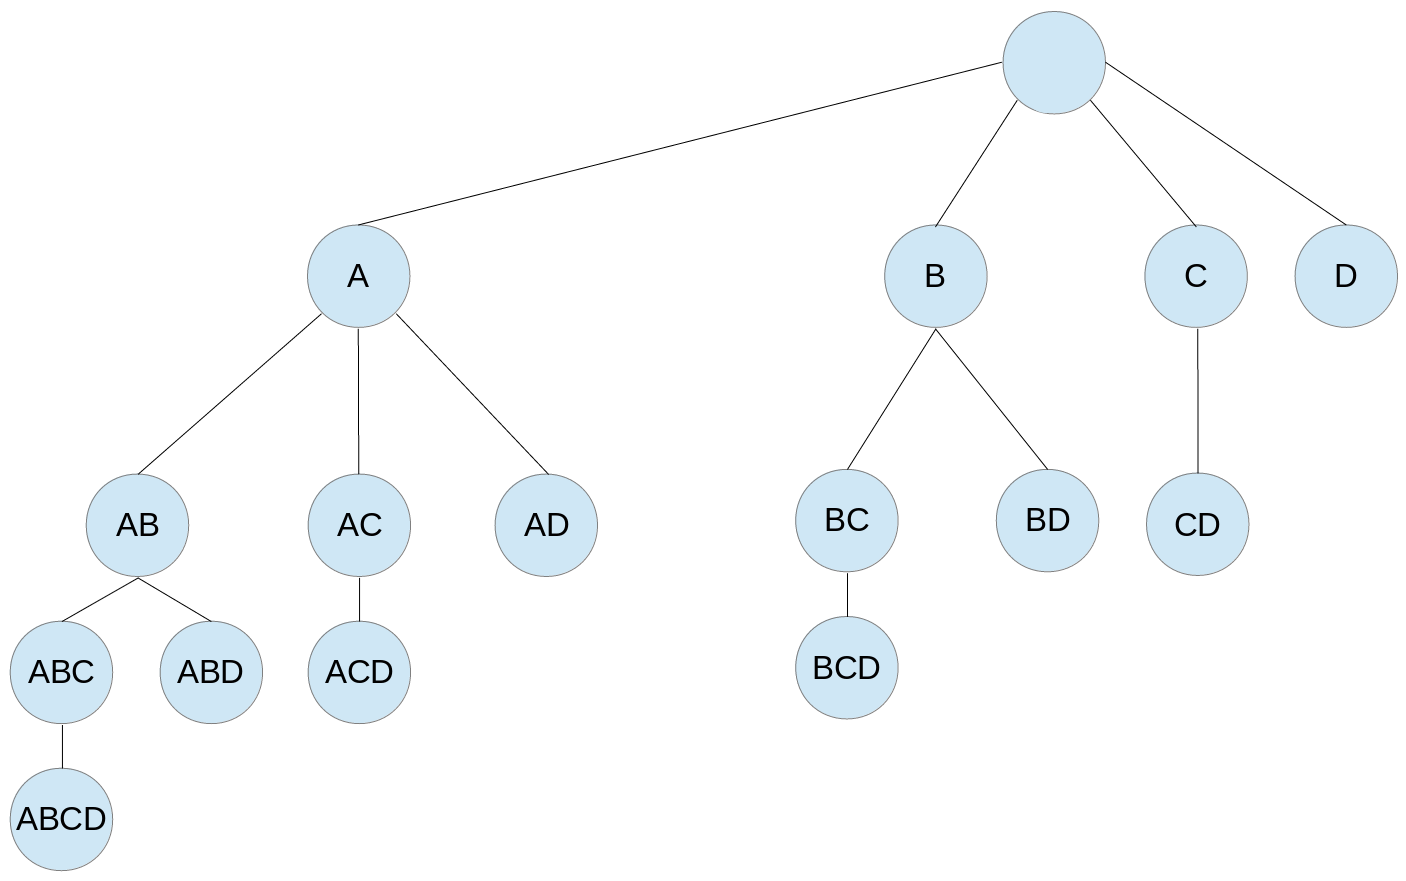
\includegraphics[width=0.7\textwidth]{figs/arvore}
\caption[Árvore de Combinações para a rede da Figura \ref{fig:grafo}.]
{Árvore de Combinações para a rede da Figura \ref{fig:grafo}.}
\label{fig:arvore}
\end{figure}

Nessa árvore, a raiz ($h=0$) é a combinação com nenhum enlace, ou seja, $C=\emptyset$ ($(|C|=0)$). Os filhos de qualquer vértice $C$ da árvore são obtidos combinando $C$ com um enlace $i \in E(G)$, tal que $i \notin C$. Para a mesma rede modelada na Figura \ref{fig:grafo}, é ilustrada sua árvore de combinações de enlaces na Figura \ref{fig:arvore}.

No contexto de árvore de combinações, é importante definir também os descendentes de um vértice. Segundo [XXX], se $P(r,v)$ é um caminho da raiz $r$ a um vértice $v$ na árvore, $v$ é descendente de $u$ se, e somente se, $u \in P(r,v)$ e $u \neq v$. Como consequência, $\forall v \in V(T)$, tal que $v \neq r$, $v$ é descendente de $r$. 

A abstração de árvore de combinações permite que os conjuntos de enlaces sejam percorridos conforme a estrutura da árvore. Com isso, é possível utilizar métodos sistemáticos para buscar e avaliar a viabilidade das combinações de enlaces. Os métodos mais famosos como Busca em Profundidade e Busca em Profundidade em árvores podem ser considerados nesse caso. Entretanto, sua utilização exige a construção prévia da árvore que apresenta alta complexidade tanto de tempo, quanto de espaço ($O(2^m)$ em ambos os casos).

Os algoritmos que serão apresentados nos próximos capítulos fazem uma busca sobre T, mas apenas usam a ideia de árvore de combinações em seus projetos. Não há construção da árvore para realizar buscas e isso representa uma diminuição considerável na complexidade de espaço. Além disso, eles fazem uso da propriedade apresentada na próxima seção que, por sua vez, ajuda a reduzir a complexidade de tempo.

\section{Modelos de Interferência}
\label{section:interference}

No capítulo \ref{cap:introducao}, os testes de interferências foram descritos de maneira intuitiva e pouco detalhada. Nessa seção, eles serão definidos formalmente e uma propriedade decorrente da natureza desses testes será apresentada. Essa propriedade é importante pois permitirá o desenvolvimento de algoritmos de enumeração com melhores desempenhos.

\subsection{Modelo de Interferência Primária}

Em \cite{primary}, a modelagem de redes sem fio é feita considerando que os enlaces são {\it half-duplex}, isto é, as antenas dos rádios dos dispositivos que compõem a rede não podem transmitir e receber mensagens ao mesmo tempo. Além disso, o transceptor em um nó apenas consegue transmitir para ou receber de um outro nó.

Em resumo, todo nó pode apenas ser transmissor ou receptor em um único enlace. Portanto, a restrição para que uma rede esteja livre de interferências primárias é que nenhum nó pode participar de mais de um enlace. Usando a abstração de grafos introduzida na seção anterior, a figura \ref{fig:primario} ilustra alguns cenários que exploram essa condição.

\begin{figure}[htb]
\centering
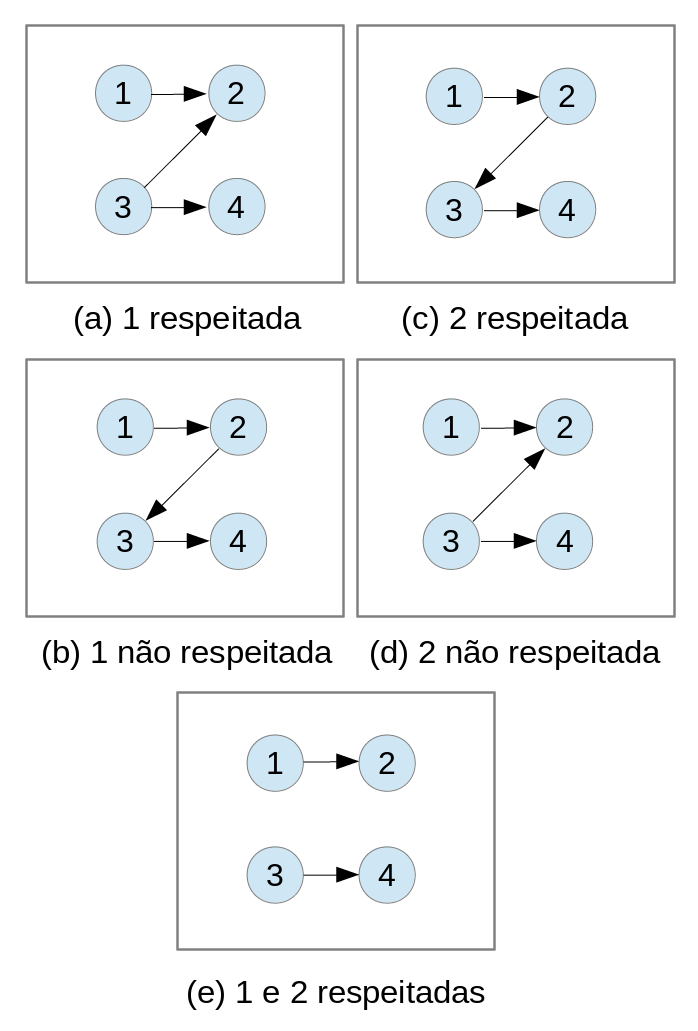
\includegraphics[width=0.7\textwidth]{figs/primario}
\caption[Cenários com diferentes variações das caraterísticas.]
{Cenários com diferentes variações das caraterísticas.}
\label{fig:primario}
\end{figure}

Na Figura \ref{fig:primario}, o cenário (a) mostra um nó transmitindo para dois outros nós ao mesmo tempo; (b) mostra um nó recebendo de dois outros nós ao mesmo tempo; (c) mostra um nó transmitindo e recebendo ao mesmo tempo; e (d), diferente dos cenários anteriores, mostra uma rede que respeita a restrição proposta.   

\subsection{Teste de Interferência Primária}

Seja $i$ um enlace de um conjunto $C \subset \mathcal{L}$. O nó transmissor e o nó receptor de $i$ são, respectivamente, $s_{i}$ e $r_{i}$. $C$ passa no Teste de Interferência Primária (TIP)\abbrev{TIP}{Teste de Interferência Primária} se, e somente se, $\forall i,j \in C, s_{i} \neq s_{j} \& s_{i} \neq r_{j} \& r_{i} \neq s_{j} \& r_{i} \neq r_{j}$. 

\begin{algorithm}[h]
	\SetVline
	{\bf input:} Conjunto de enlaces $C$\\
	\ForEach { $i \in C$}{
		\ForEach { $j \in C$, $j \neq i$}{
			\If { (( $s_{i}==s_{j}$ ) $||$ ( $s_{i}==r_{j}$ ) $||$ ( $r_{i}==s_{j}$ ) $||$ ( $r_{i}==r_{j}$ ))}{
				\Return FALSE
			}
		}
	}
	\Return TRUE
\caption{Algoritmo TIP}
\label{alg:tip}
\end{algorithm}

\subsubsection{Prova de Corretude}

O TIP apenas formaliza o que foi definido na subseção anterior. Portanto, o algoritmo está correto. 

\subsubsection{Análise da Complexidade}

Para o pior caso, $|C|=m$, então a complexidade de tempo é $O(m^2)$. A complexidade de espaço é definida pelo maior tamanho de $C$ possível, portanto, $O(m)$.

\subsection{Modelo de Interferência Secundária}

O Modelo de Interferência Secundária é definido em \cite{sinr, models}. Nesse modelo, é considerada uma grandeza chamada SINR ({\it Signal to Interference plus Noise Ratio}) \abbrev{SINR}{Signal to Interference plus Noise Ratio} que representa uma razão entre o sinal recebido e as interferências sofridas por um nó.

Conforme discutido na Seção \ref{section:mesh}, nesse trabalho é usado o modelo de propagação {\it log-distance}. A potência de recepão $PR(s,r)$ de um sinal transmitido por $s$ e recebido por $r$ é definido como,

\begin{equation}
PR(s,r) = \frac{PT}{(\frac{d_{sr}}{d_{0}})^{\alpha}}
\label{eq:rp}
\end{equation}

onde $\alpha$ é o coeficiente e $d_{0}$ é a distância de referência do modelo de propagação.

Para um enlace $i$, dado um nó receptor $r_{i}$, consegue-se calcular a potência de recepção em $r_{i}$ em duas situações distintas:

\begin{itemize} %verificar se pode ter lista com 2 itens

\item quando o sinal é transmitido por $s_{i}$, ou seja, é a potência de recepção dentro do próprio enlace $i$; 
\item quando o sinal é transmitido por $s_{j}$, tal que $j \neq i$, ou seja, é a potência de recepção de um sinal transmitido em um outro enlace $j$. Nesse caso, a potência de recepção de tais sinais é chamada de interferência. 

\end{itemize}

A interferência será analisada entre os enlaces que compõem um conjunto $C$. Com isso, denomina-se Interferência Total $I(i,C)$ a soma das interferências que os nós transmissores de todos os outros enlaces de $C$ exercem sobre o nó receptor do enlace $i$. Ou seja,

\begin{equation}
I(i,C) = \sum_{j \neq i} PR(s_{j},r_{i})
\end{equation}

Finalmente, a $SINR(i,C)$ é a razão entre a potência de recepção em $r_{i}$ referente a transmissão no enlace $i$ e a soma do ruído do ambiente $\gamma$ com a interferência total dos outros enlaces no conjunto $C$.

\begin{equation}
SINR(i,C) = \frac{PR(s_{i},r_{i})} {\gamma + I(i,C)}
\label{eq:sinr}  
\end{equation}

Dado um conjunto de enlaces $C$ e tendo calculado $SINR(i,C)$, $\forall i \in C$, compara-se os valores encontrados com uma constante $\beta$, que representa um valor numérico para o limite de interferência tolerado. Se a interferência for muito alta, o valor do denominador na Equação~\ref{eq:sinr} irá aumentar, fazendo o valor da $SINR(i,C)$ diminuir. 

\subsection{Teste de Interferência Secundária}

No modelo de interferência secundária, $\beta$ é um limite inferior, tal que, se $SINR(i,C) \geq \beta$ , $\forall i \in C$, então $C$ passa no Teste de Interferência Secundária (TIS)\abbrev{TIS}{Teste de Interferência Secundária}.

\subsubsection{Descrição do Algoritmo}

\begin{algorithm}[h]
	\SetVline
	{\bf input:} Conjunto de enlaces $C$\\
	\ForEach { $i \in C$}{
		\If {(( $SINR(i,C)<\beta$ ))}{
			\Return FALSE
		}
	}
	\Return TRUE
\caption{Algoritmo TIS}
\label{alg:tis}
\end{algorithm}

\subsubsection{Prova de Corretude}

O TIS apenas formaliza o que foi definido na subseção 2.2.2. Portanto, está correto.

\subsubsection{Análise da Complexidade}

Como itera-se sobre todos os enlaces de C para calcular $SINR(i,C)$, sua complexidade é $O(m)$. Devido o laço definido na linha 2 iterar sobre no máximo m enlaces, então a complexidade de tempo é $O(m^2)$. Analogamente ao TIP, a complexidade de espaço é $O(m)$.

\subsection{Viabilidade de Conjuntos}

Dados os modelos de interferência apresentados, se um conjunto de enlace $C$ passar em ambos os testes, então diz-se que $C$ é viável. Essa definição é apresentada em \cite{scheduling}. O algoritmo para testar a viabilidade de um conjunto de enlaces é simplesmente a junção dos algoritmos anteriores.

\subsubsection{Descrição do Algoritmo}

\begin{algorithm}[h]
	\SetVline
	{\bf input:} Conjunto de enlaces $C$\\
		\If { (TIP(C)) $\&\&$ (TIS(C))}{
			\Return TRUE
		}
		\Else {
			\Return FALSE
		}
\caption{Algoritmo VIAVEL}
\label{alg:viavel}
\end{algorithm}

\subsubsection{Prova de Corretude}

A condicional da linha 2 garante que ambos os testes são executados e, somente ao passar necessariamente nos dois, um conjunto C é classificado como viável. Portanto, o algoritmo está correto.

\subsubsection{Análise da Complexidade}

O pior caso para o teste de viabilidade é quando o conjunto é viável, ou seja, todas as iterações do TIP e do TIS ocorrem. Para o maior tamanho de C possível, temos que a complexidade de tempo desse algoritmo é $O(m)+O(m^2)=O(m^2)$.

\subsection{Inviabilidade Hereditária}

Dados os modelos de interferência apresentados, se um conjunto de enlace $C$ passar em ambos os testes, então diz-se que $C$ é viável. Entretanto, nesta subseção, será analisado o que acontece quando C não é viável.

Em um primeiro cenário, assume-se que $C$ não passou no TIP. Nesse caso, pelo menos um nó de $C$ está participando de mais de um enlace, o que é proibido. Seja um conjunto $C'$, tal que $C' = C \cup \{i\}$, onde $i \in E$. A adição do novo enlace $i$ em $C$ pode: ({\bf i}) conectar dois nós contidos em $C$; ({\bf ii}) conectar um nó existente em $C$ a um novo nó; e ({\bf iii}) incluir dois novos nós conectados por $i$. 
  
Nas três situações descritas anteriormente, a adição do novo enlace $i$ para formar $C'$ não muda o fato de que $C$ não é viável, independentemente do efeito que $i$ cause no conjunto original $C$. Consequentemente, é possível notar que $C'$ também não é viável.

Em um segundo cenário, assume-se que $C$ passou no TIP, mas não passou no TIS. Nesse caso, $SINR(i,C) < \beta$, para algum enlace $i$. Seja um conjunto $C'$, tal que, $C' = C \cup \{j\}$, onde $j \in E$ e $C'$ também passa no TIP. A adição de um novo enlace ao conjunto $C$ para formar $C'$, apenas fará aumentar a interferência nos enlaces já contidos em $C$. Mesmo que a contribuição na interferência total seja pequena, podendo até ser desprezada, a adição de um novo enlace não muda o fato de que $C$ não é viável. Consequentemente, é possível notar que $C'$ também não é viável.

Os dois cenários apresentados garantem a seguinte propriedade: se um conjunto $C$ não é viável, independentemente de qual teste de interferência ele falhou, então qualquer conjunto $C'$, tal que $C \subset C'$ também não é viável. Usando o modelo de árvore de combinações apresentado na seção anterior, se uma combinação $C$ da árvore de combinações não é viável, então todos os seus descendentes na árvore também não são viáveis. Por isso, essa propriedade é denominada Inviabilidade Hereditária. 

Devido a Inviabilidade Hereditária, no processo de busca e verificação de viabilidade de todas as combinações de enlaces de uma rede, sabe-se que, ao encontrar qualquer combinação não viável, não é necessário testar a viabilidade de nenhum de seus descendentes. O ato de não testar os descendentes de uma combinação não viável pode ser chamado de ``podar'' a árvore. 

\section{Exemplo com Busca em Profundidade}
\label{section:bp}

A rede modelada na Figura \ref{fig:grafo} será utilizada para construir esse exemplo. O objetivo é encontrar os conjuntos de enlaces viáveis dessa rede. 

Nesse exemplo, os nós foram distribuídos aleatoriamente em uma área quadrada de lado $2000m$. As potências de transmissão foram fixadas em $PT=350mW=24.7712dBm$ para todos os nós. Nesse cenário, $m=4$ enlaces foram definidos, $E(G)=\{A, B, C, D\}$. Uma descrição dos enlaces contendo a distância entre os nós e a potência de recepção pode ser encontrada na Tabela \ref{table:enlaces}. Os valores do coeficiente e da distância de referência do modelo de propagação utilizados foram, respectivamente, $\alpha=4,0$ e $d_0=1,0$m.

\begin{table}[h]
\centering
\caption[Descrição dos Enlaces.]
{Descrição dos Enlaces.}
\label{table:enlaces}
\begin{tabular}{lccc}
\hline
Enlace & Distância ($m$) & Potência de Recepção ($10^{-8}mW$)\\ \hline
A=(4,3)	& $322,583$	& $2,77047$\\
B=(2,1)	& $292,245$	& $4,11274$\\
C=(2,3)	& $192,006$	& $22,0730$\\
D=(5,6)	& $179,399$	& $28,9628$
\end{tabular}
\end{table}

Existem $2^4 = 16$ combinações de enlaces que são representados na árvore de combinações da Figura \ref{fig:bp}. Uma Busca em Profundidade será executada para percorrer os vértices da árvore que serão verificados usando o algoritmo VIÁVEL. A ordem em que os vértices são visitados é $\{\{\}, \{A\}, \{A,B\}, \{A,B,C\}, \{A,B,C,D\}, \{A,B,D\}, \{A,C\}, \{A,C,D\}, \{A,D\},$ $\{B\}, \{B,C\}, \{B,C,D\},$ $\{B,D\}, \{C\}, \{C,D\}, \{D\}\}$ e pode ser verificada também na Figura \ref{fig:bp}. A Tabela \ref{table:resultadoviabilidade} mostra o resultado dos testes para cada combinação. 

\begin{figure}[htb]
\centering
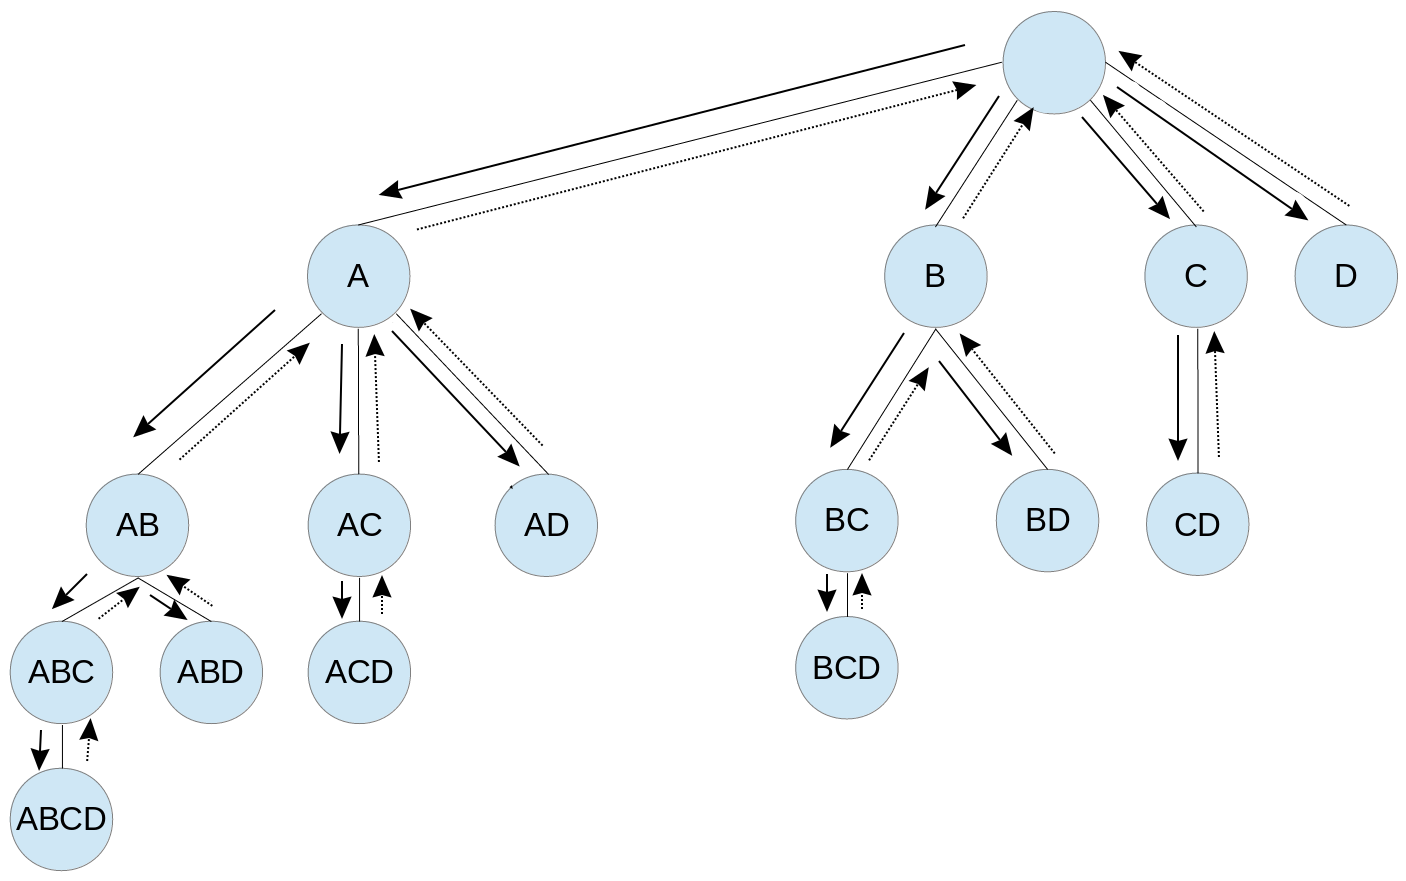
\includegraphics[width=1\textwidth]{figs/bp}
\caption[Busca em Profundidade na árvore de combinações.]
{Busca em Profundidade na árvore de combinações.}
\label{fig:bp}
\end{figure}

\begin{table}[h]
\centering
\caption[Resultados dos Testes de Viabilidade.]
{Resultados dos Testes de Viabilidade.}
\label{table:resultadoviabilidade}
\begin{tabular}{lcc}
\hline
Conjunto & Situação\\ \hline
\{\} & Dispensa teste\\
\{A\}	& Dispensa teste\\
\{A,B\}	& Falha TIS\\
\{A,B,C\}	& "Podado"\\
\{A,B,C,D\}	& "Podado"\\
\{A,B,D\}	& "Podado"\\
\{A,C\}	& Falha TIP\\
\{A,C,D\}	& "Podado"\\
\{A,D\}	& Falha TIS\\
\{B\}	& Dispensa teste\\
\{B,C\}	& Falha TIP\\
\{B,C,D\}	& "Podado"\\
\{B,D\}	& OK\\
\{C\}	& Dispensa teste\\
\{C,D\}	& OK\\
\{D\}	& Dispensa teste\\
\end{tabular}
\end{table}

O conjunto vazio e os conjuntos com apenas 1 enlace dispensam o teste de viabilidade. O primeiro conjunto a ser testado de verdade é o conjunto \{A,B\} que é reprovado no TIS e, portanto seus descendentes serão "podados". O conjunto \{A,C\} é reprovado no TIP pois A e C compartilham o nó 3 e, com isso, \{A,C,D\} é "podado". Em seguida, \{A,D\} é testado e reprovado no TIS, mas como é uma folha da árvore, a busca continua normalmente, sem "poda". O conjunto \{B,C\} é testado e reprovado no TIP pois B e C compartilham o nó 2 e, consequentemente, \{B,C,D\} é "podado". Finalmente, os conjuntos \{B,D\} e \{C,D\} são testados e classificados como viáveis, já que passam em ambos os testes.
Conclui-se que os conjuntos de enlaces viáveis obtidos são: $\{\{\},\{A\},\{B\},\{B,D\},\{C\},\{C,D\},\{D\}\}$. 

\begin{table}[H]
\centering
\caption{Cálculos das SINR}
\label{table:sinr}
\begin{tabular}{|c|l|c|c|c|}
\hline
\multicolumn{1}{|l|}{Combinação} & Enlaces($i=s_i,r_i$) & \multicolumn{1}{l|}{$d(s_j,r_i)${[}m{]}} & \multicolumn{1}{l|}{$I(j,i)[10^{-11}$mW$]$} & \multicolumn{1}{l|}{$SINR(i, \{i,j\}$){[}mW{]}} \\ \hline
                                 & C=(4,6)          & 1263,04                              & 11,7883                                  & \cellcolor[HTML]{9AFF99}1.115,22962           \\ \cline{2-5} 
\multirow{-2}{*}{\{C,D\}}        & D=(5,6)          & 1590,92                              & 4,68303                                  & \cellcolor[HTML]{9AFF99}2.282,86418           \\ \hline
                                 & B=(2,1)          & 1744,24                              & 3,24112                                  & \cellcolor[HTML]{9AFF99}365,73588             \\ \cline{2-5} 
\multirow{-2}{*}{\{B,D\}}        & D=(5,6)          & 1590,92                              & 4,68303                                  & \cellcolor[HTML]{9AFF99}2.282,86418           \\ \hline
                                 & A=(4,3)          & 1263,04                              & 11,78830                                 & \cellcolor[HTML]{FFCCC9}\textbf{139,97729}    \\ \cline{2-5} 
\multirow{-2}{*}{\{A,D\}}        & D=(5,6)          & 1327,55                              & 9,65865                                  & \cellcolor[HTML]{9AFF99}1.639,77421           \\ \hline
                                 & A=(4,3)          & 192,006                              & 22073,0                                  & \cellcolor[HTML]{FFCCC9}\textbf{0,12547}      \\ \cline{2-5} 
\multirow{-2}{*}{\{A,B\}}        & B=(2,1)          & 673,016                              & 146,224                                  & \cellcolor[HTML]{FFCCC9}\textbf{26,66666}     \\ \hline
\end{tabular}
\end{table}

A justificativa dos resultados dos TIS realizados são mostrados na Figura \ref{table:sinr}. O valor da tolerância de interferência escolhido foi $\beta=316,228$mW. A coluna das distâncias $d(s_j,r_i)$ mostra a distância entre transmissor de j ao receptor de i. Baseada nessa distância, a interferência total $I(j,i)$ na próxima coluna foi calculada. Na última coluna, o valor das {$SINR(i, \{i,j\}$  calculadas são listadas. Aquelas com valores menores que $\beta$ estão sombreadas de vermelho e justificam a combinação relacionada não ter passado no TIS. Para o cálculo da {$SINR(i, \{i,j\}$, o valor do ruído do ambiente utilizado foi $\gamma=8,004 \times 10^{-11}$ mW.

%No Apêndice A, é apresentada a justificativa para a escolha de todos os parâmetros para o Modelo de Interferência Secundária. Os parâmetros usados para construir esse exemplo também foram utilizados na parte de implementação para gerar as redes usadas nos experimentos. 

\section{Vantagens e Desvantagens}
\label{section:complexity}

No pior caso, o processo de enumeração descrito na seção anterior percorre todos os $2^m$ vértices da árvore, aplicando VIAVEL em cada conjunto de enlaces. Isso representa uma complexidade de $O(2^mm^2)$. Na prática, as redes possuem uma densidade grande. Por isso, é um exagero assumir que $2^m$ combinações serão testadas, pois certamente haverão muitos conjuntos não viáveis. 

Seja F o conjunto de combinações viáveis obtido por meio de um processo de enumeração como o da seção anterior. Certamente, $|F|$ combinações foram testadas, caso contrário não fariam parte de F. Na maioria dos casos, os conjuntos não viáveis são "podados" de forma que só um primeiro conjunto é testado. Supondo o pior caso, sempre depois de um conjunto viável com maior altura em um ramo da árvore ser testado, encontra-se um conjunto não viável. Nesse caso, o número de combinações testadas é igual a $|F| + |U|$, onde U é o conjunto das primeiras combinações não viáveis testadas depois de uma viável. É possível ver que $|F| \approx |U|$ e, portanto, o número de conjuntos testados é $2|F|$. 

Existe, então, um bom candidato a substituir a porção exponencial da complexidade do algoritmo mencionado. Como $O(|F|)$ conjuntos serão testados (viáveis ou não), a complexidade pode ser alterada para $O(|F|m^2)$. Até o momento, $|F|$ é desconhecido, mas certamente varia em função do tamanho da rede. No Capítulo \ref{cap:resultados}, uma função que represente os valores de $|F|$ usando m e n como parâmetros é aproximada, definindo melhor o valor da complexidade.

Mesmo com uma potencial redução da complexidade de tempo ao utilizar o valor $|F|$, a complexidade de espaço desse algoritmo ainda é exponencial. Isso significa que sua implementação está limitada a pequenos valores de m.

\section{Conclusão}
\label{section:conclusion}
Nesse capítulo, todo o problema foi modelado usando diferentes abstrações com o intuito de obter um procedimento sistemático para enumerar combinações viáveis. Devido a essa modelagem, a complexidade de tempo encontrada em algoritmos que usam força bruta pode ser modificada para um valor diferente, que será estudado em capítulos futuros. Ainda assim, a complexidade de espaço continua exponencial, inviabilizando sua utilização na maioria das aplicações.

